\documentclass{article}
\usepackage{pgfplots}
\pgfplotsset{compat=newest}

\begin{document}

\begin{figure}[h]
    \centering
    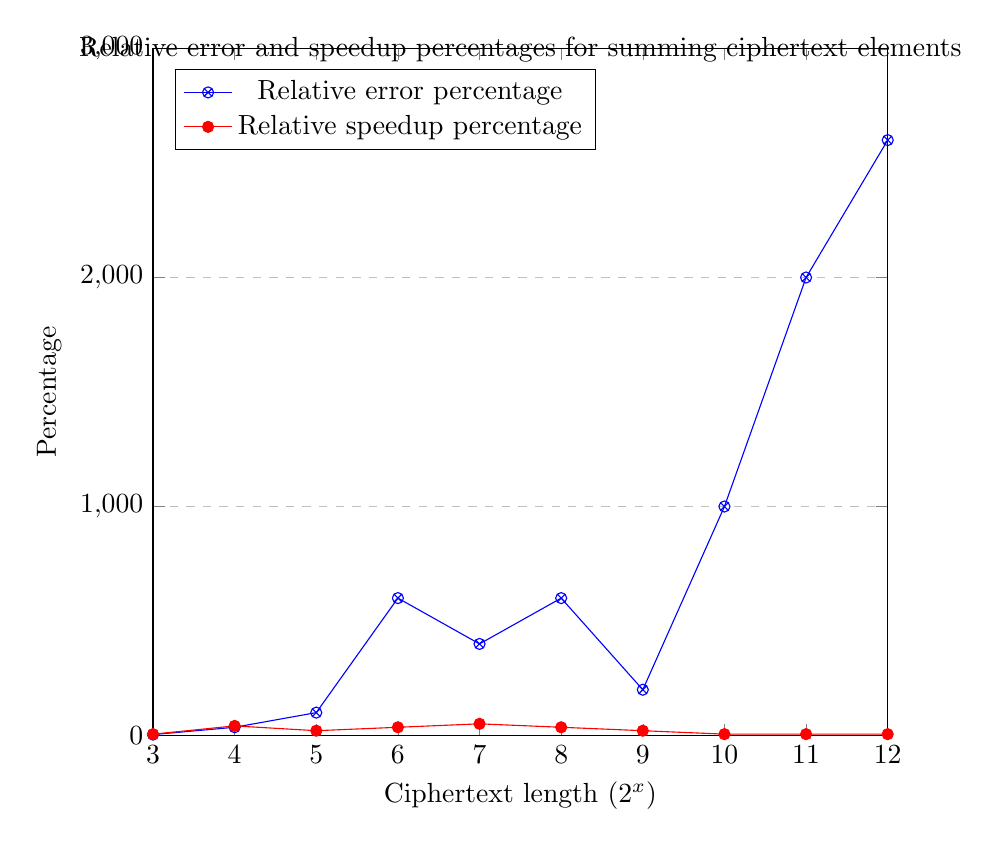
\begin{tikzpicture}
        \begin{axis}[
            width=0.9\textwidth,
            height=0.85\textwidth,
            xlabel={Ciphertext length ($2^x$)},
            ylabel={Percentage},
            xmin=3, xmax=12,
            ymin=0, ymax=3000,
            xtick=data,
            ytick={0, 1000, 2000, 3000},
            legend pos=north west,
            ymajorgrids=true,
            grid style=dashed,
            title style={yshift=-5mm},
            title={Relative error and speedup percentages for summing ciphertext elements},
        ]
            \addplot[
                color=blue,
                mark=otimes,
                ]
                coordinates {
                    (3, 4)(4, 36)(5, 100)(6, 600)(7, 400)(8, 600)(9, 200)(10, 1000)(11, 2000)(12, 2600)
                };
            \addlegendentry{Relative error percentage}
            
            \addplot[
                color=red,
                mark=*,
                ]
                coordinates {
                    (3, 6)(4, 42)(5, 21)(6, 36)(7, 51)(8, 36)(9, 21)(10, 6)(11, 6)(12, 6)
                };
            \addlegendentry{Relative speedup percentage}
        \end{axis}
    \end{tikzpicture}
    \caption{Relative error and speedup percentages for summing ciphertext elements using DFT vs RA (Rotate and Add).}
    \label{fig:relative_error_speedup}
\end{figure}

Summation of ciphertext elements can be performed using two methods - (i) Discrete Fourier Transform (DFT); (ii) Rotate and Add (RA). This plot (\ref{fig:relative_error_speedup}) depicts the relative error percentage and relative speedup percentage of these methods for various ciphertext lengths in summing ciphertext elements. The relative error percentage is calculated as:
\[
\text{Relative error percentage} = \left(\frac{\text{DFT} - \text{RA}}{\text{RA}}\right) \times 100.
\]
The relative speedup percentage is calculated as:
\[
\text{Relative speedup percentage} = \left(\frac{T_{DFT} - T_{RA}}{T_{RA}}\right) \times 100,
\]
where \( T \) denotes the time taken using the respective method.
\end{document}